% Generated by LitigCharts.PublicationFigures. Captions and provenance are sidecars.
\documentclass[10pt,tikz,border=5pt]{standalone}
\usepackage{lmodern}
\usetikzlibrary{patterns,patterns.meta}
\begin{document}
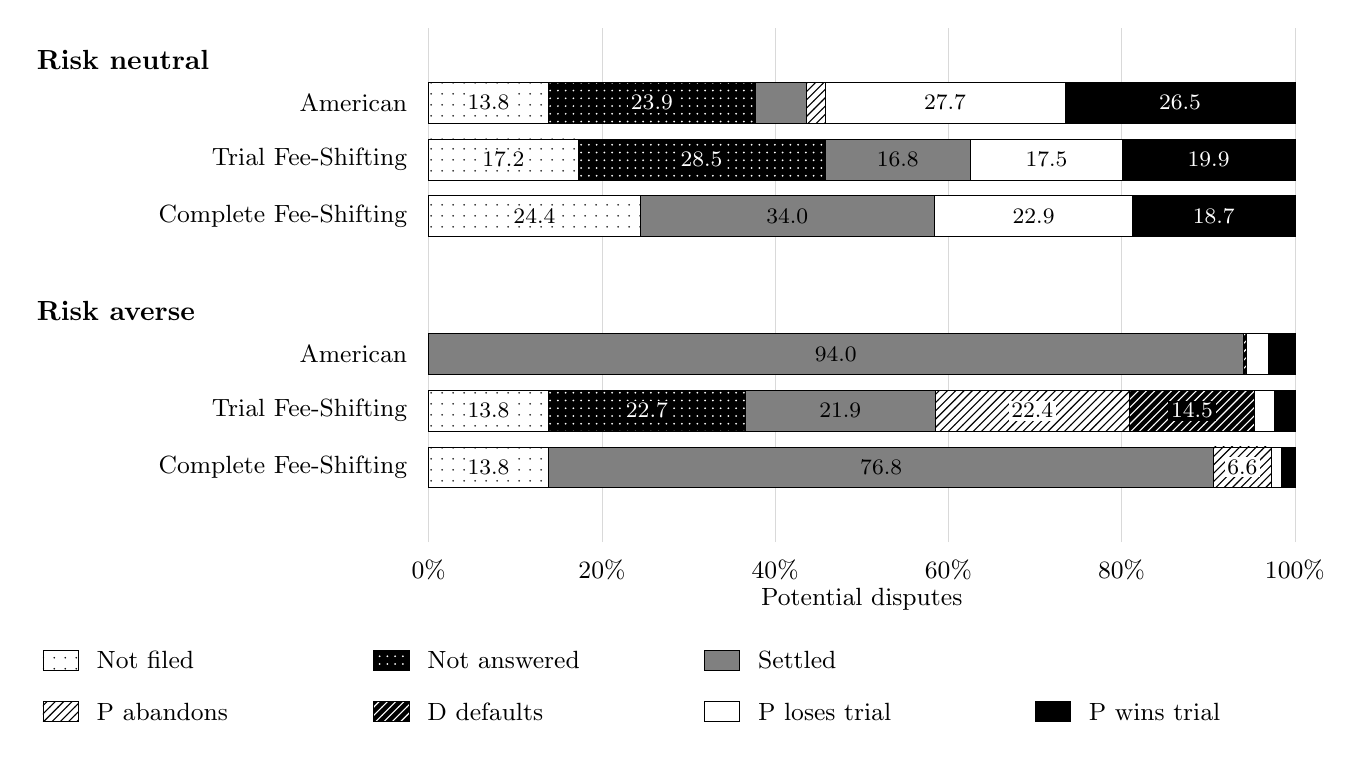
\begin{tikzpicture}[font=\small]\draw[black!15,line width=.2pt] (5.1,.65) -- (5.1,7.18);
\node[anchor=north] at (5.1,.55) {0\%};
\draw[black!15,line width=.2pt] (7.3,.65) -- (7.3,7.18);
\node[anchor=north] at (7.3,.55) {20\%};
\draw[black!15,line width=.2pt] (9.5,.65) -- (9.5,7.18);
\node[anchor=north] at (9.5,.55) {40\%};
\draw[black!15,line width=.2pt] (11.7,.65) -- (11.7,7.18);
\node[anchor=north] at (11.7,.55) {60\%};
\draw[black!15,line width=.2pt] (13.9,.65) -- (13.9,7.18);
\node[anchor=north] at (13.9,.55) {80\%};
\draw[black!15,line width=.2pt] (16.1,.65) -- (16.1,7.18);
\node[anchor=north] at (16.1,.55) {100\%};
\node[anchor=west,font=\bfseries] at (0,6.78) {\mbox{Risk} \mbox{neutral}};
\node[anchor=east] at (4.95,6.23) {American};
\path[preaction={fill=white,draw=none},pattern={Dots[distance=4pt,radius=.35pt]},pattern color=black,draw=black,line width=.25pt] (5.1,5.97) rectangle (6.62141,6.49);
\node[text=black,fill=white,font=\footnotesize,inner sep=1pt] at (5.860705,6.23) {13.8};
\path[preaction={fill=black,draw=none},pattern={Dots[distance=2.8pt,radius=.35pt]},pattern color=white,draw=black,line width=.25pt] (6.62141,5.97) rectangle (9.247924,6.49);
\node[text=white,fill=black,font=\footnotesize,inner sep=1pt] at (7.934667,6.23) {23.9};
\path[fill=black!50,draw=black,line width=.25pt] (9.247924,5.97) rectangle (9.891692,6.49);
\path[preaction={fill=white,draw=none},pattern={north east lines},pattern color=black,draw=black,line width=.25pt] (9.891692,5.97) rectangle (10.131442,6.49);
\path[fill=white,draw=black,line width=.25pt] (10.131442,5.97) rectangle (13.183722,6.49);
\node[text=black,fill=none,font=\footnotesize,inner sep=1pt] at (11.657582,6.23) {27.7};
\path[fill=black,draw=black,line width=.25pt] (13.183722,5.97) rectangle (16.100009,6.49);
\node[text=white,fill=none,font=\footnotesize,inner sep=1pt] at (14.641865,6.23) {26.5};
\node[anchor=east] at (4.95,5.51) {Trial Fee-Shifting};
\path[preaction={fill=white,draw=none},pattern={Dots[distance=4pt,radius=.35pt]},pattern color=black,draw=black,line width=.25pt] (5.1,5.25) rectangle (6.996367,5.77);
\node[text=black,fill=white,font=\footnotesize,inner sep=1pt] at (6.048184,5.51) {17.2};
\path[preaction={fill=black,draw=none},pattern={Dots[distance=2.8pt,radius=.35pt]},pattern color=white,draw=black,line width=.25pt] (6.996367,5.25) rectangle (10.133017,5.77);
\node[text=white,fill=black,font=\footnotesize,inner sep=1pt] at (8.564692,5.51) {28.5};
\path[fill=black!50,draw=black,line width=.25pt] (10.133017,5.25) rectangle (11.980841,5.77);
\node[text=black,fill=none,font=\footnotesize,inner sep=1pt] at (11.056929,5.51) {16.8};
\path[fill=white,draw=black,line width=.25pt] (11.980841,5.25) rectangle (13.909856,5.77);
\node[text=black,fill=none,font=\footnotesize,inner sep=1pt] at (12.945349,5.51) {17.5};
\path[fill=black,draw=black,line width=.25pt] (13.909856,5.25) rectangle (16.1,5.77);
\node[text=white,fill=none,font=\footnotesize,inner sep=1pt] at (15.004928,5.51) {19.9};
\node[anchor=east] at (4.95,4.79) {Complete Fee-Shifting};
\path[preaction={fill=white,draw=none},pattern={Dots[distance=4pt,radius=.35pt]},pattern color=black,draw=black,line width=.25pt] (5.1,4.53) rectangle (7.78499,5.05);
\node[text=black,fill=white,font=\footnotesize,inner sep=1pt] at (6.442495,4.79) {24.4};
\path[fill=black!50,draw=black,line width=.25pt] (7.78499,4.53) rectangle (11.524275,5.05);
\node[text=black,fill=none,font=\footnotesize,inner sep=1pt] at (9.654633,4.79) {34.0};
\path[fill=white,draw=black,line width=.25pt] (11.524275,4.53) rectangle (14.040448,5.05);
\node[text=black,fill=none,font=\footnotesize,inner sep=1pt] at (12.782362,4.79) {22.9};
\path[fill=black,draw=black,line width=.25pt] (14.040448,4.53) rectangle (16.1,5.05);
\node[text=white,fill=none,font=\footnotesize,inner sep=1pt] at (15.070224,4.79) {18.7};
\node[anchor=west,font=\bfseries] at (0,3.59) {\mbox{Risk} \mbox{averse}};
\node[anchor=east] at (4.95,3.04) {American};
\path[fill=black!50,draw=black,line width=.25pt] (5.1,2.78) rectangle (15.440671,3.3);
\node[text=black,fill=none,font=\footnotesize,inner sep=1pt] at (10.270336,3.04) {94.0};
\path[preaction={fill=black,draw=none},pattern={north east lines},pattern color=white,draw=black,line width=.25pt] (15.440671,2.78) rectangle (15.484412,3.3);
\path[fill=white,draw=black,line width=.25pt] (15.484412,2.78) rectangle (15.763493,3.3);
\path[fill=black,draw=black,line width=.25pt] (15.763493,2.78) rectangle (16.1,3.3);
\node[anchor=east] at (4.95,2.32) {Trial Fee-Shifting};
\path[preaction={fill=white,draw=none},pattern={Dots[distance=4pt,radius=.35pt]},pattern color=black,draw=black,line width=.25pt] (5.1,2.06) rectangle (6.62141,2.58);
\node[text=black,fill=white,font=\footnotesize,inner sep=1pt] at (5.860705,2.32) {13.8};
\path[preaction={fill=black,draw=none},pattern={Dots[distance=2.8pt,radius=.35pt]},pattern color=white,draw=black,line width=.25pt] (6.62141,2.06) rectangle (9.120907,2.58);
\node[text=white,fill=black,font=\footnotesize,inner sep=1pt] at (7.871159,2.32) {22.7};
\path[fill=black!50,draw=black,line width=.25pt] (9.120907,2.06) rectangle (11.532888,2.58);
\node[text=black,fill=none,font=\footnotesize,inner sep=1pt] at (10.326898,2.32) {21.9};
\path[preaction={fill=white,draw=none},pattern={north east lines},pattern color=black,draw=black,line width=.25pt] (11.532888,2.06) rectangle (13.997614,2.58);
\node[text=black,fill=white,font=\footnotesize,inner sep=1pt] at (12.765251,2.32) {22.4};
\path[preaction={fill=black,draw=none},pattern={north east lines},pattern color=white,draw=black,line width=.25pt] (13.997614,2.06) rectangle (15.588995,2.58);
\node[text=white,fill=black,font=\footnotesize,inner sep=1pt] at (14.793305,2.32) {14.5};
\path[fill=white,draw=black,line width=.25pt] (15.588995,2.06) rectangle (15.8393,2.58);
\path[fill=black,draw=black,line width=.25pt] (15.8393,2.06) rectangle (16.100002,2.58);
\node[anchor=east] at (4.95,1.6) {Complete Fee-Shifting};
\path[preaction={fill=white,draw=none},pattern={Dots[distance=4pt,radius=.35pt]},pattern color=black,draw=black,line width=.25pt] (5.1,1.34) rectangle (6.62141,1.86);
\node[text=black,fill=white,font=\footnotesize,inner sep=1pt] at (5.860705,1.6) {13.8};
\path[fill=black!50,draw=black,line width=.25pt] (6.62141,1.34) rectangle (15.071137,1.86);
\node[text=black,fill=none,font=\footnotesize,inner sep=1pt] at (10.846274,1.6) {76.8};
\path[preaction={fill=white,draw=none},pattern={north east lines},pattern color=black,draw=black,line width=.25pt] (15.071137,1.34) rectangle (15.797341,1.86);
\node[text=black,fill=white,font=\footnotesize,inner sep=1pt] at (15.434239,1.6) {6.6};
\path[fill=white,draw=black,line width=.25pt] (15.797341,1.34) rectangle (15.93025,1.86);
\path[fill=black,draw=black,line width=.25pt] (15.93025,1.34) rectangle (16.1,1.86);
\node at (10.6,-.08) {Potential disputes};
\path[preaction={fill=white,draw=none},pattern={Dots[distance=4pt,radius=.35pt]},pattern color=black,draw=black,line width=.25pt] (0.2,-0.98) rectangle (0.65,-0.72);
\node[anchor=west] at (0.76,-0.85) {Not filed};
\path[preaction={fill=black,draw=none},pattern={Dots[distance=2.8pt,radius=.35pt]},pattern color=white,draw=black,line width=.25pt] (4.4,-0.98) rectangle (4.85,-0.72);
\node[anchor=west] at (4.96,-0.85) {Not answered};
\path[fill=black!50,draw=black,line width=.25pt] (8.6,-0.98) rectangle (9.05,-0.72);
\node[anchor=west] at (9.16,-0.85) {Settled};
\path[preaction={fill=white,draw=none},pattern={north east lines},pattern color=black,draw=black,line width=.25pt] (0.2,-1.63) rectangle (0.65,-1.37);
\node[anchor=west] at (0.76,-1.5) {P abandons};
\path[preaction={fill=black,draw=none},pattern={north east lines},pattern color=white,draw=black,line width=.25pt] (4.4,-1.63) rectangle (4.85,-1.37);
\node[anchor=west] at (4.96,-1.5) {D defaults};
\path[fill=white,draw=black,line width=.25pt] (8.6,-1.63) rectangle (9.05,-1.37);
\node[anchor=west] at (9.16,-1.5) {P loses trial};
\path[fill=black,draw=black,line width=.25pt] (12.8,-1.63) rectangle (13.25,-1.37);
\node[anchor=west] at (13.36,-1.5) {P wins trial};
\end{tikzpicture}
\end{document}
